\chapter{Research Methodology}\label{ch:research-methodology}
%\lipsum[2-8]
\initial{F}rom the literature there is a clear lack of results for localisation systems using the commercial Pozyx sensor network with drones in an household environment.
To address the aims and objectives stated in ~\ref{sec:aims_objs}, it is proposed that a lightweight on-board localisation be developed to check the feasibility of minimal hardware solution for an indoor drone.
This would entail connecting a Pozyx tag directly to a FCU and integrate it with the pose localisation system existing already.
To close the loop the pose information should be available in some format that can be used for autonomous control.
Furthermore, the system should be tested in a practical environment, to this end, the Pozyx anchor network was setup in a kitchen.
A kitchen represents one of the highest traffic areas in a household and it contains various materials that will make raw readings from a UWB system noisy and inaccurate.
As a kitchen will contain both dynamic and static obstacles multiple anchor configurations must be tested in order to find optimal anchor positions in this given environment.

\section{Anchor Configurations}\label{sec:anchor-configurations}
Noting work from ~\citet{di2019evaluation} and the setup procedures from ~\citet{pozyx2018pozyx} it is important to have at least 4 anchors setup in non-planar orientations for the best positioning results.
To determine a suitable anchor configuration in the given space a tag was placed at fixed known point in a given reference frame and the mounted locations of the 4 anchors were varied on each wall of the kitchen in order to prevent planar configurations and ambiguity when the tag calculates its position.
Figure ~\ref{fig:layout} shows a simplified layout and toybox configuration of the tag and anchors.
Grey areas represent areas in the space that is impossible to traverse, red represents known obstacles that interfere and attenuate the UWB signal, blue represent anchors, green the tag, cream is partially obstructed and the rest of the area is fully traversable.
Before each run and data collection the tag was manually configured with the location of each of the anchors in the reference frame of the kitchen and recorded for at least 5 seconds.
The tag was triggered to calculate the position repeatedly within the timeframe and the function call is blocking and takes $\approx70ms$ so data was recorded at a frequency of $\approx14.28Hz$.
With a tag position of (1480,2330,980)mm, the following statistics were calculated using Matlab.
In addition to the average error and standard deviation,  kurtosis and skew metrics were added to show the number of outliers and symmetry of the recorded data.
The error metrics are important to give an idea of how noisy the overall data is while kurtosis and skewness gives an indication if the noise follows a uniform distribution which would be beneficial ideal for state estimators.
From table ~\ref{tb:config_stats} we can see that configuration 12 gives acceptable error metrics and reasonable skew and kurtosis making it the best out of the configurations tested.
To further support this Figure ~\ref{fig:config} shows several results obtained with several configurations and it can be seen that configuration 12 produced the best results with minimal noise and measurment outliers as well as it was centered around the ground truth position of the tag.

\begin{figure}[h!]
    \centering
    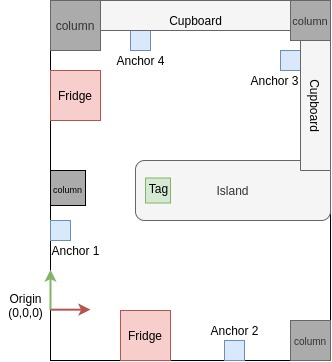
\includegraphics{mtd/Kitchen_layout}
    \caption{Birds eye view of the test environment.}
    \label{fig:layout}
\end{figure}
\newpage

\begin{longtable}[h!]{| c | c |}
    \hline
    Config & Anchor positions (mm)$\left(\begin{array}{c}
   Anchor1(x,y,z),\\Anchor2(x,y,z),\\Anchor3(x,y,z),\\ Anchor4(x,y,z)
   \end{array}\right)$ \\
    \hline
    1 & $\left(\begin{array}{c}
   (0,0,1115),\\(3680, -405, 1550),\\(3655, 4080, 1906),\\(270, 4465, 2090)
   \end{array}\right)$\\
    \hline
    2 & $\left(\begin{array}{c}
   (0,665,1115),\\(2995, -405, 1889),\\(3655, 4080, 1906),\\(270, 4465, 2090)
   \end{array}\right)$\\
    \hline
    3 & $\left(\begin{array}{c}
   (0,665,1115),\\(2995, -405, 1889),\\(3655, 4080, 1906),\\(1526, 4559, 837)
   \end{array}\right)$\\
    \hline
    4 & $\left(\begin{array}{c}
   (0,665,1115),\\(2995, -405, 1889),\\(3655, 4080, 1906),\\(1070, 5170, 491)
   \end{array}\right)$\\
    \hline
    5 & $\left(\begin{array}{c}
   (0,665,1115),\\(2995, -405, 1889),\\(3960, 3368, 2304),\\(1070, 5170, 491)
   \end{array}\right)$\\
    \hline
    6 & $\left(\begin{array}{c}
   (0,665,1115),\\(2737, -410, 1913),\\(3655, 3598, 1668),\\(1187, 4760, 590)
   \end{array}\right)$\\
    \hline
    7 & $\left(\begin{array}{c}
   (0,665,1115),\\(2737, -410, 1913),\\(3655, 4529, 1777),\\(1187, 4760, 590)
   \end{array}\right)$\\
    \hline
    8 & $\left(\begin{array}{c}
   (0,645,1214),\\(2737, -410, 1913),\\(3651, 4120, 1853),\\(1066, 4760, 491)
   \end{array}\right)$\\
    \hline
    9 & $\left(\begin{array}{c}
   (0,645,1214),\\(2737, -410, 1913),\\(3970, 3063, 2320),\\(1066, 4760, 491)
   \end{array}\right)$\\
    \hline
    10 & $\left(\begin{array}{c}
   (0,645,1214),\\(2737, -410, 1913),\\(3651, 3550, 1810),\\(1066, 4760, 491)
   \end{array}\right)$\\
   \hline
    11 & $\left(\begin{array}{c}
   (0,645,1214),\\(2737, -410, 1913),\\(3651, 3550, 1810),\\(1591, 4450, 1775)
   \end{array}\right)$\\
    \hline
    \rowcolor{LightGreen}12 & $\left(\begin{array}{c}
   (0,645,1214),\\(2737, -410, 1913),\\(3651, 4120, 1853),\\(1591, 4450, 1775)
   \end{array}\right)$\\
    \hline
    \caption{Anchor locations for each Configuration}
    \label{tb:ach_loc}
\end{longtable}

%\begin{table}[h!]
   \begin{longtable}[h!]{| c | c | c | c | c |}
       \hline
       Config
       & Avg. Error & Std. Deviation$\left(\begin{array}{c}
       x,\\y,\\z
       \end{array}\right)$ & Kurtosis & Skewness\\
       \hline
       1 & 342.5906 & $\left(\begin{array}{c}
       183.1707,\\205.3426,\\972.6239
       \end{array}\right)$&$\left( \begin{array}{c}
       2.349,\\ 1.5967,\\ 1.415
       \end{array} \right)$&$\left( \begin{array}{c}
       -0.4083,\\ -0.3522,\\ 0.4551
       \end{array} \right)$\\
       \hline
              2 &  173.5938 & $\left(\begin{array}{c}
       43.2345,\\45.6897,\\133.8616\\
       \end{array}\right)$&$\left( \begin{array}{c}
       21.8923,\\ 10.1765,\\ 119.1344
       \end{array} \right)$&$\left( \begin{array}{c}
       -2.8672,\\ -0.3453,\\ 8.9025
       \end{array} \right)$\\
       \hline
              3 &  203.8502 & $\left(\begin{array}{c}
       128.4693,\\118.3216,\\209.1637
       \end{array}\right)$&$\left( \begin{array}{c}
       14.2955,\\ 11.2045,\\ 2.9124
       \end{array} \right)$&$\left( \begin{array}{c}
       -2.579,\\  -0.3920,\\ 0.4055
       \end{array} \right)$\\
       \hline
              4 &  85.8562 & $\left(\begin{array}{c}
       40.2197,\\40.6081,\\66.2120
       \end{array}\right)$&$\left( \begin{array}{c}
       6.7558,\\ 7.5180,\\ 3.4722
       \end{array} \right)$&$\left( \begin{array}{c}
       -0.4260,\\ -0.5344,\\ -0.1242
       \end{array} \right)$\\
       \hline
              5 &  64.8616 & $\left(\begin{array}{c}
       65.3883,\\53.8458,\\78.5751
       \end{array}\right)$&$\left( \begin{array}{c}
       13.3707,\\ 13.2178,\\ 11.0111
       \end{array} \right)$&$\left( \begin{array}{c}
       -0.6016,\\ 0.3745,\\ 0.0461
       \end{array} \right)$\\
       \hline
              6 &  189.933 & $\left(\begin{array}{c}
       40.8435,\\32.6482,\\58.5618
       \end{array}\right)$&$\left( \begin{array}{c}
       11.8957,\\ 11.8924,\\ 11.092
       \end{array} \right)$&$\left( \begin{array}{c}
       0.7516,\\ -0.0100,\\ -0.1322
       \end{array} \right)$\\
       \hline
              7 &  100.6929 & $\left(\begin{array}{c}
       75.8269,\\72.0940,\\41.9398
       \end{array}\right)$&$\left( \begin{array}{c}
       26.0285,\\ 17.4295,\\ 7.2328
       \end{array} \right)$&$\left( \begin{array}{c}
       -3.1681,\\ -0.8384,\\ -0.7151
       \end{array} \right)$\\
       \hline
              8 &  138.1276 & $\left(\begin{array}{c}
       26.2243,\\21.8750,\\70.6189
       \end{array}\right)$&$\left( \begin{array}{c}
       4.6048,\\ 52.2374,\\ 50.9467
       \end{array} \right)$&$\left( \begin{array}{c}
       -0.4858,\\ 5.0752,\\ 5.1757
       \end{array} \right)$\\
       \hline
              9 &  258.296 & $\left(\begin{array}{c}
       165.7105,\\95.081,\\475.0623
       \end{array}\right)$&$\left( \begin{array}{c}
       2.2833,\\ 1.7939,\\ 2.3406
       \end{array} \right)$&$\left( \begin{array}{c}
       -0.6982,\\ 0.2746,\\ 0.7517
       \end{array} \right)$\\
       \hline
              10 &  235.348 & $\left(\begin{array}{c}
       116.1306,\\89.9868,\\420.8322
       \end{array}\right)$&$\left( \begin{array}{c}
       3.6670,\\ 4.7058,\\ 3.8066
       \end{array} \right)$&$\left( \begin{array}{c}
       1.5079,\\ -1.7613,\\ -1.5615
       \end{array} \right)$\\
       \hline
              11 &  223.4468 & $\left(\begin{array}{c}
       120.9674,\\79.8602,\\409.8192
       \end{array}\right)$&$\left( \begin{array}{c}
       3.389,\\ 4.6663,\\ 3.1988
       \end{array} \right)$&$\left( \begin{array}{c}
       1.1099,\\ -1.5397,\\ -1.2038
       \end{array} \right)$\\
       \hline
              \rowcolor{LightGreen}12 &  111.8493 & $\left(\begin{array}{c}
       27.568,\\17.7124,\\64.4278
       \end{array}\right)$&$\left( \begin{array}{c}
       4.8522,\\ 7.4335,\\ 6.2489
       \end{array} \right)$&$\left( \begin{array}{c}
       -0.0239,\\ -0.8535,\\ 3.7132
       \end{array} \right)$\\
       \hline
       \caption{Statistics of the data recorded for each configuration.}
        \label{tb:config_stats}
   \end{longtable}
%\end{table}

    \begin{figure}[h!]
        \centering
        \begin{subfigure}[b]{0.49\textwidth}
            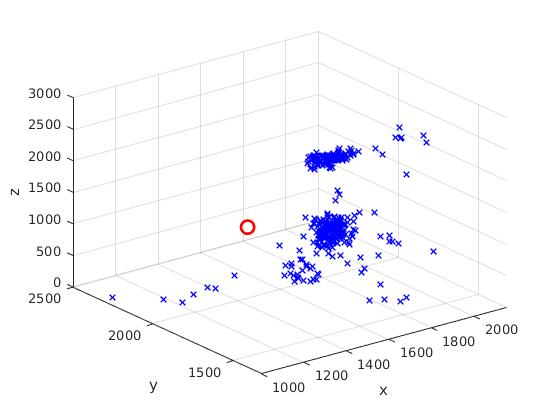
\includegraphics[width=\textwidth]{results/config1}
            \caption{Plot of Config 1}
        \end{subfigure}
        ~ %add desired spacing between images, e. g. ~, \quad, \qquad, \hfill etc.
          %(or a blank line to force the subfigure onto a new line)
        \begin{subfigure}[b]{0.49\textwidth}
            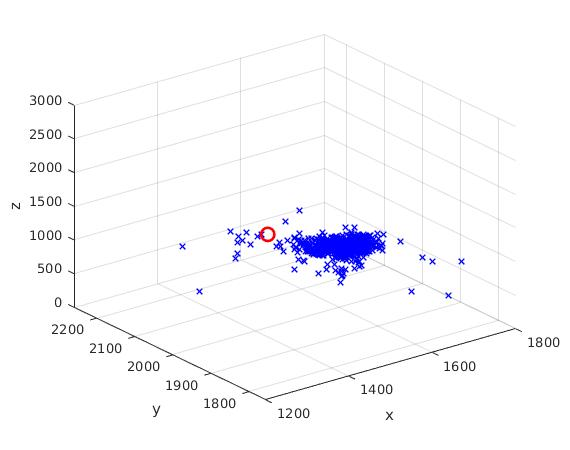
\includegraphics[width=\textwidth]{results/config2}
            \caption{Plot of Config 2}
        \end{subfigure}

        \begin{subfigure}[b]{0.49\textwidth}
            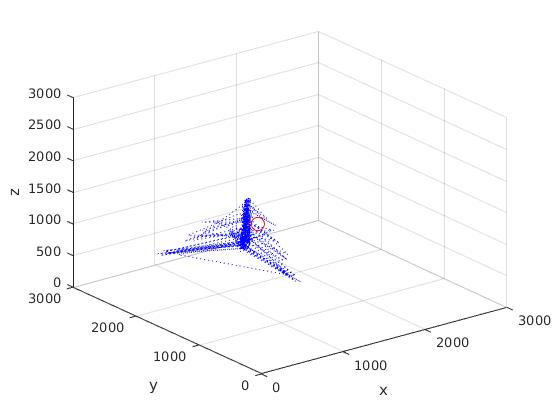
\includegraphics[width=\textwidth]{results/config3}
            \caption{Plot of Config 3}
        \end{subfigure}
        ~ %add desired spacing between images, e. g. ~, \quad, \qquad, \hfill etc.
          %(or a blank line to force the subfigure onto a new line)
        \begin{subfigure}[b]{0.49\textwidth}
            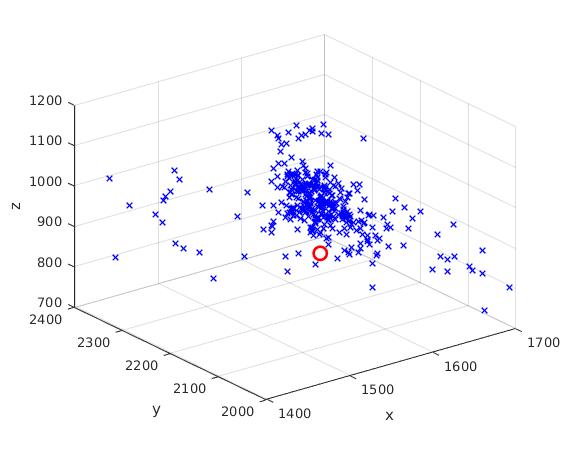
\includegraphics[width=\textwidth]{results/config4}
            \caption{Plot of Config 4}
        \end{subfigure}

        \begin{subfigure}[b]{0.49\textwidth}
            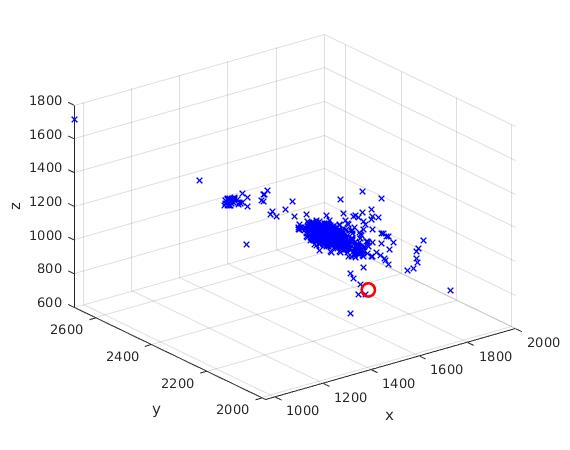
\includegraphics[width=\textwidth]{results/config5}
            \caption{Plot of Config 5}
        \end{subfigure}
        ~ %add desired spacing between images, e. g. ~, \quad, \qquad, \hfill etc.
          %(or a blank line to force the subfigure onto a new line)
        \begin{subfigure}[b]{0.49\textwidth}
            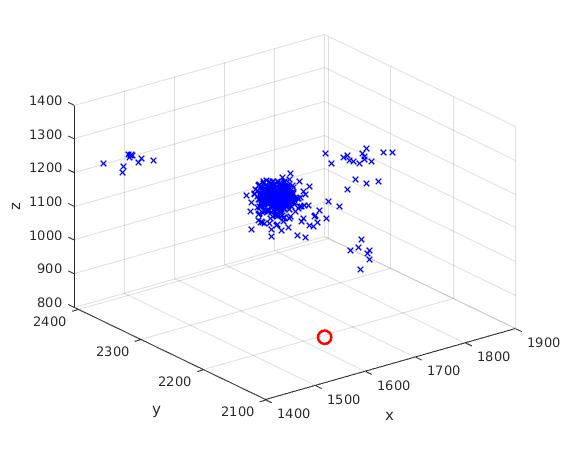
\includegraphics[width=\textwidth]{results/config6}
            \caption{Plot of Config 6}
        \end{subfigure}
        \caption{Sample plots of several anchor configurations.}
        \label{fig:config}
    \end{figure}

    \begin{figure}\ContinuedFloat
        \begin{subfigure}[b]{0.49\textwidth}
            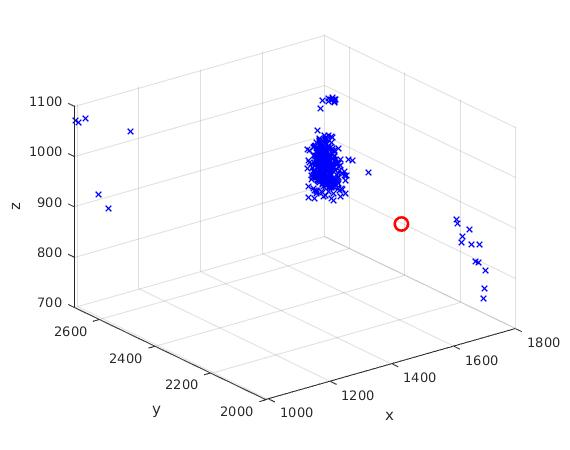
\includegraphics[width=\textwidth]{results/config7}
            \caption{Plot of Config 7}
        \end{subfigure}
        ~ %add desired spacing between images, e. g. ~, \quad, \qquad, \hfill etc.
          %(or a blank line to force the subfigure onto a new line)
        \begin{subfigure}[b]{0.49\textwidth}
            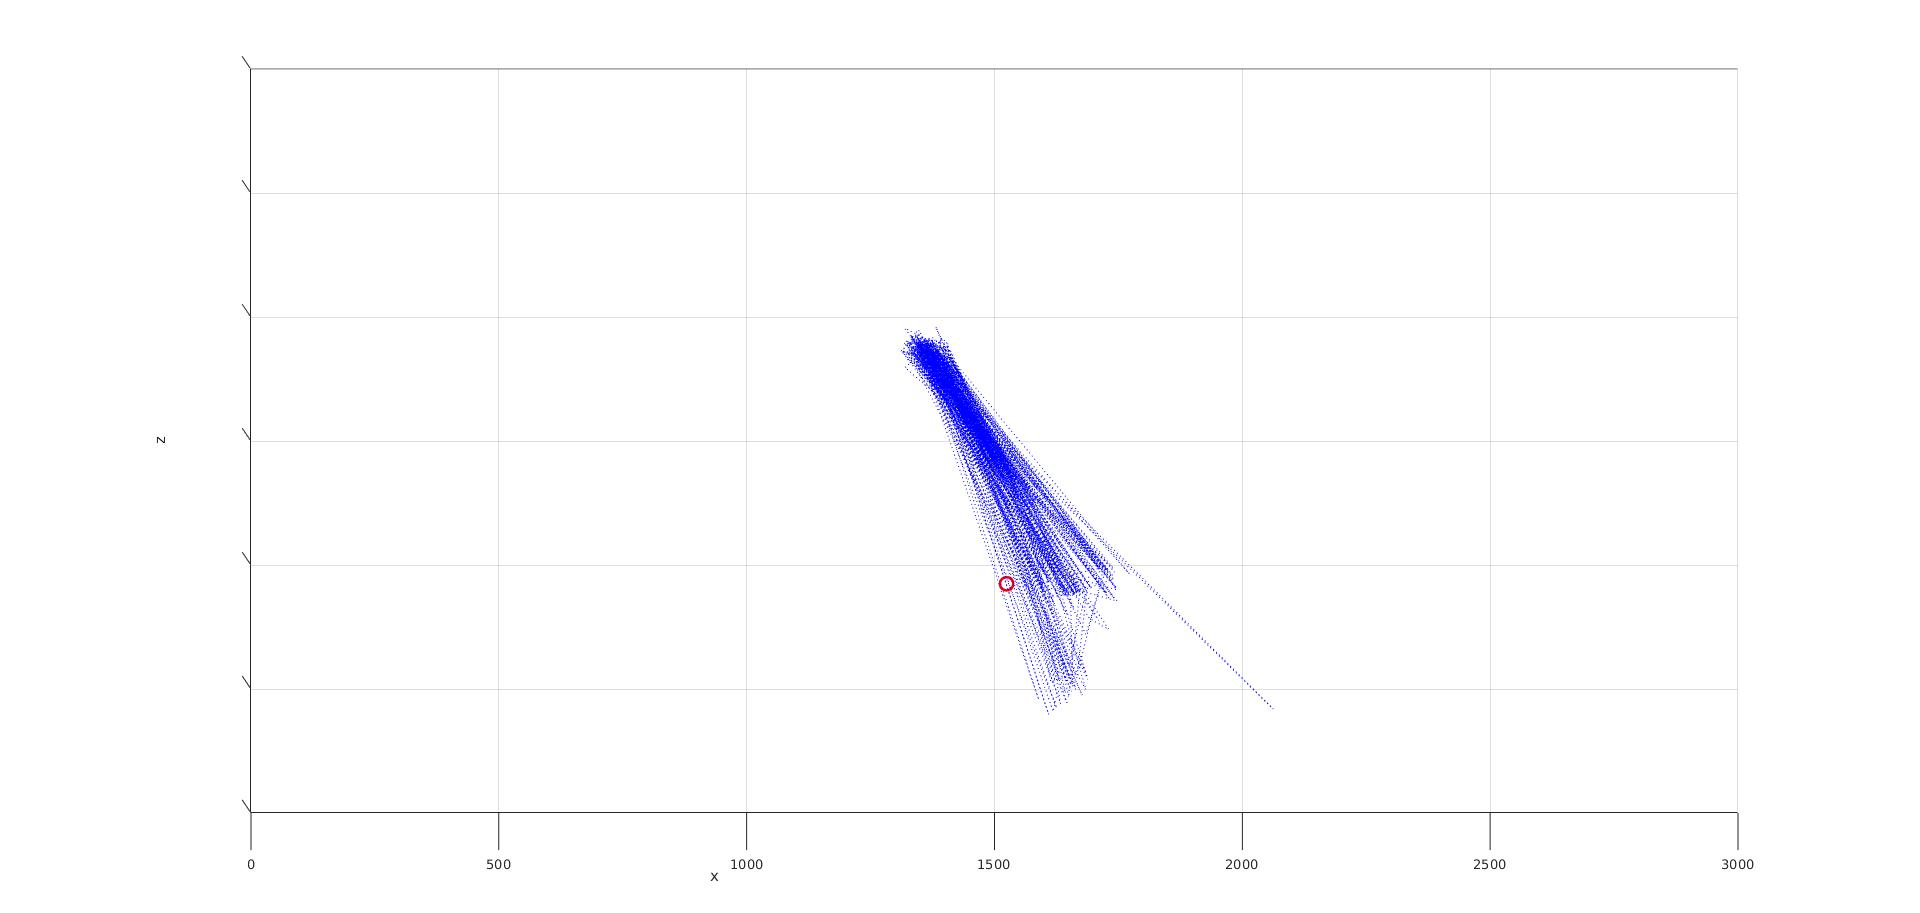
\includegraphics[width=\textwidth]{results/config8}
            \caption{Plot of Config 8}
        \end{subfigure}

        \begin{subfigure}[b]{0.49\textwidth}
            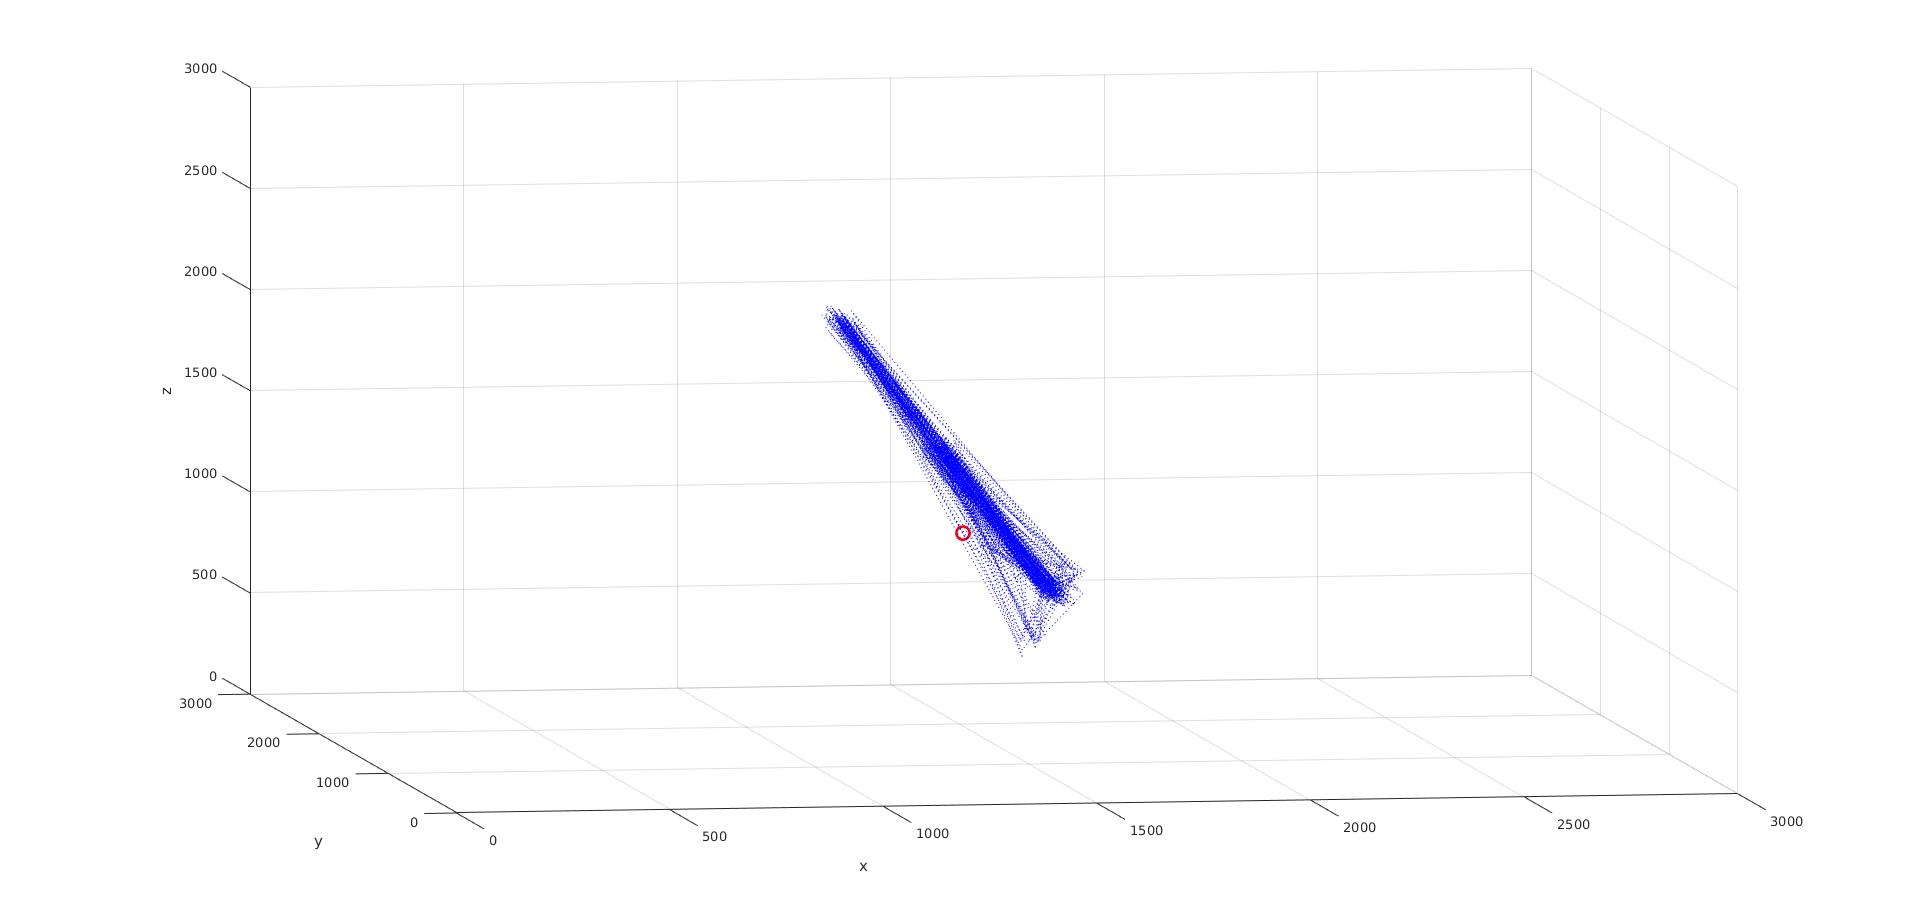
\includegraphics[width=\textwidth]{results/config9}
            \caption{Plot of Config 9}
        \end{subfigure}
        ~ %add desired spacing between images, e. g. ~, \quad, \qquad, \hfill etc.
          %(or a blank line to force the subfigure onto a new line)
        \begin{subfigure}[b]{0.49\textwidth}
            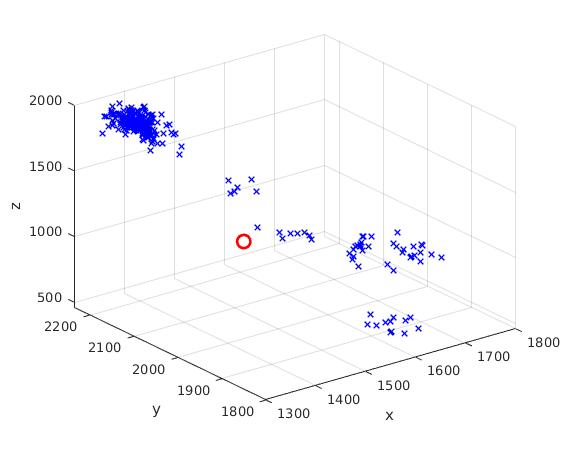
\includegraphics[width=\textwidth]{results/config10}
            \caption{Plot of Config 10}
        \end{subfigure}

        \begin{subfigure}[b]{0.49\textwidth}
            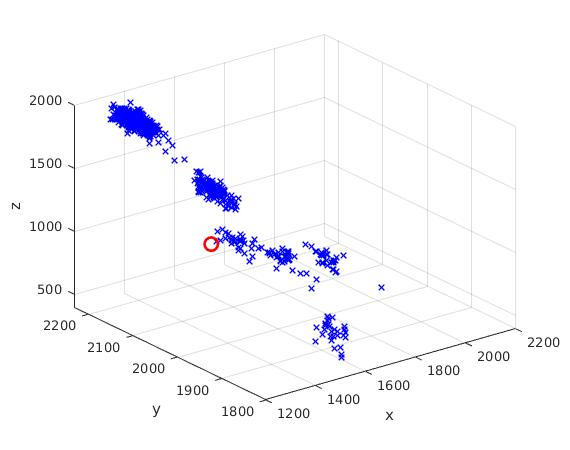
\includegraphics[width=\textwidth]{results/config11}
            \caption{Plot of Config 11}
        \end{subfigure}
        ~ %add desired spacing between images, e. g. ~, \quad, \qquad, \hfill etc.
          %(or a blank line to force the subfigure onto a new line)
        \begin{subfigure}[b]{0.49\textwidth}
            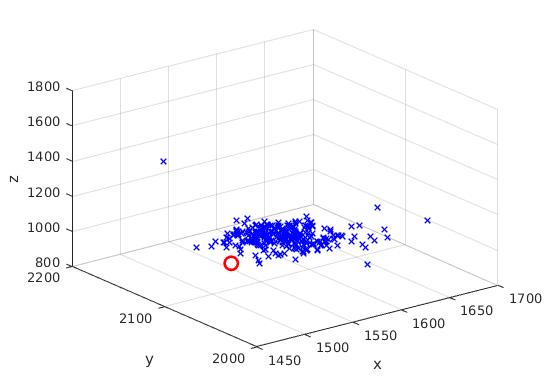
\includegraphics[width=\textwidth]{results/config12}
            \caption{Plot of Config 12}
        \end{subfigure}
        \caption[]{Sample plots of several anchor configurations. (cont'd)}
    \end{figure}


\begin{figure}[h!]
    \centering
    \begin{subfigure}[b]{0.4\textwidth}
            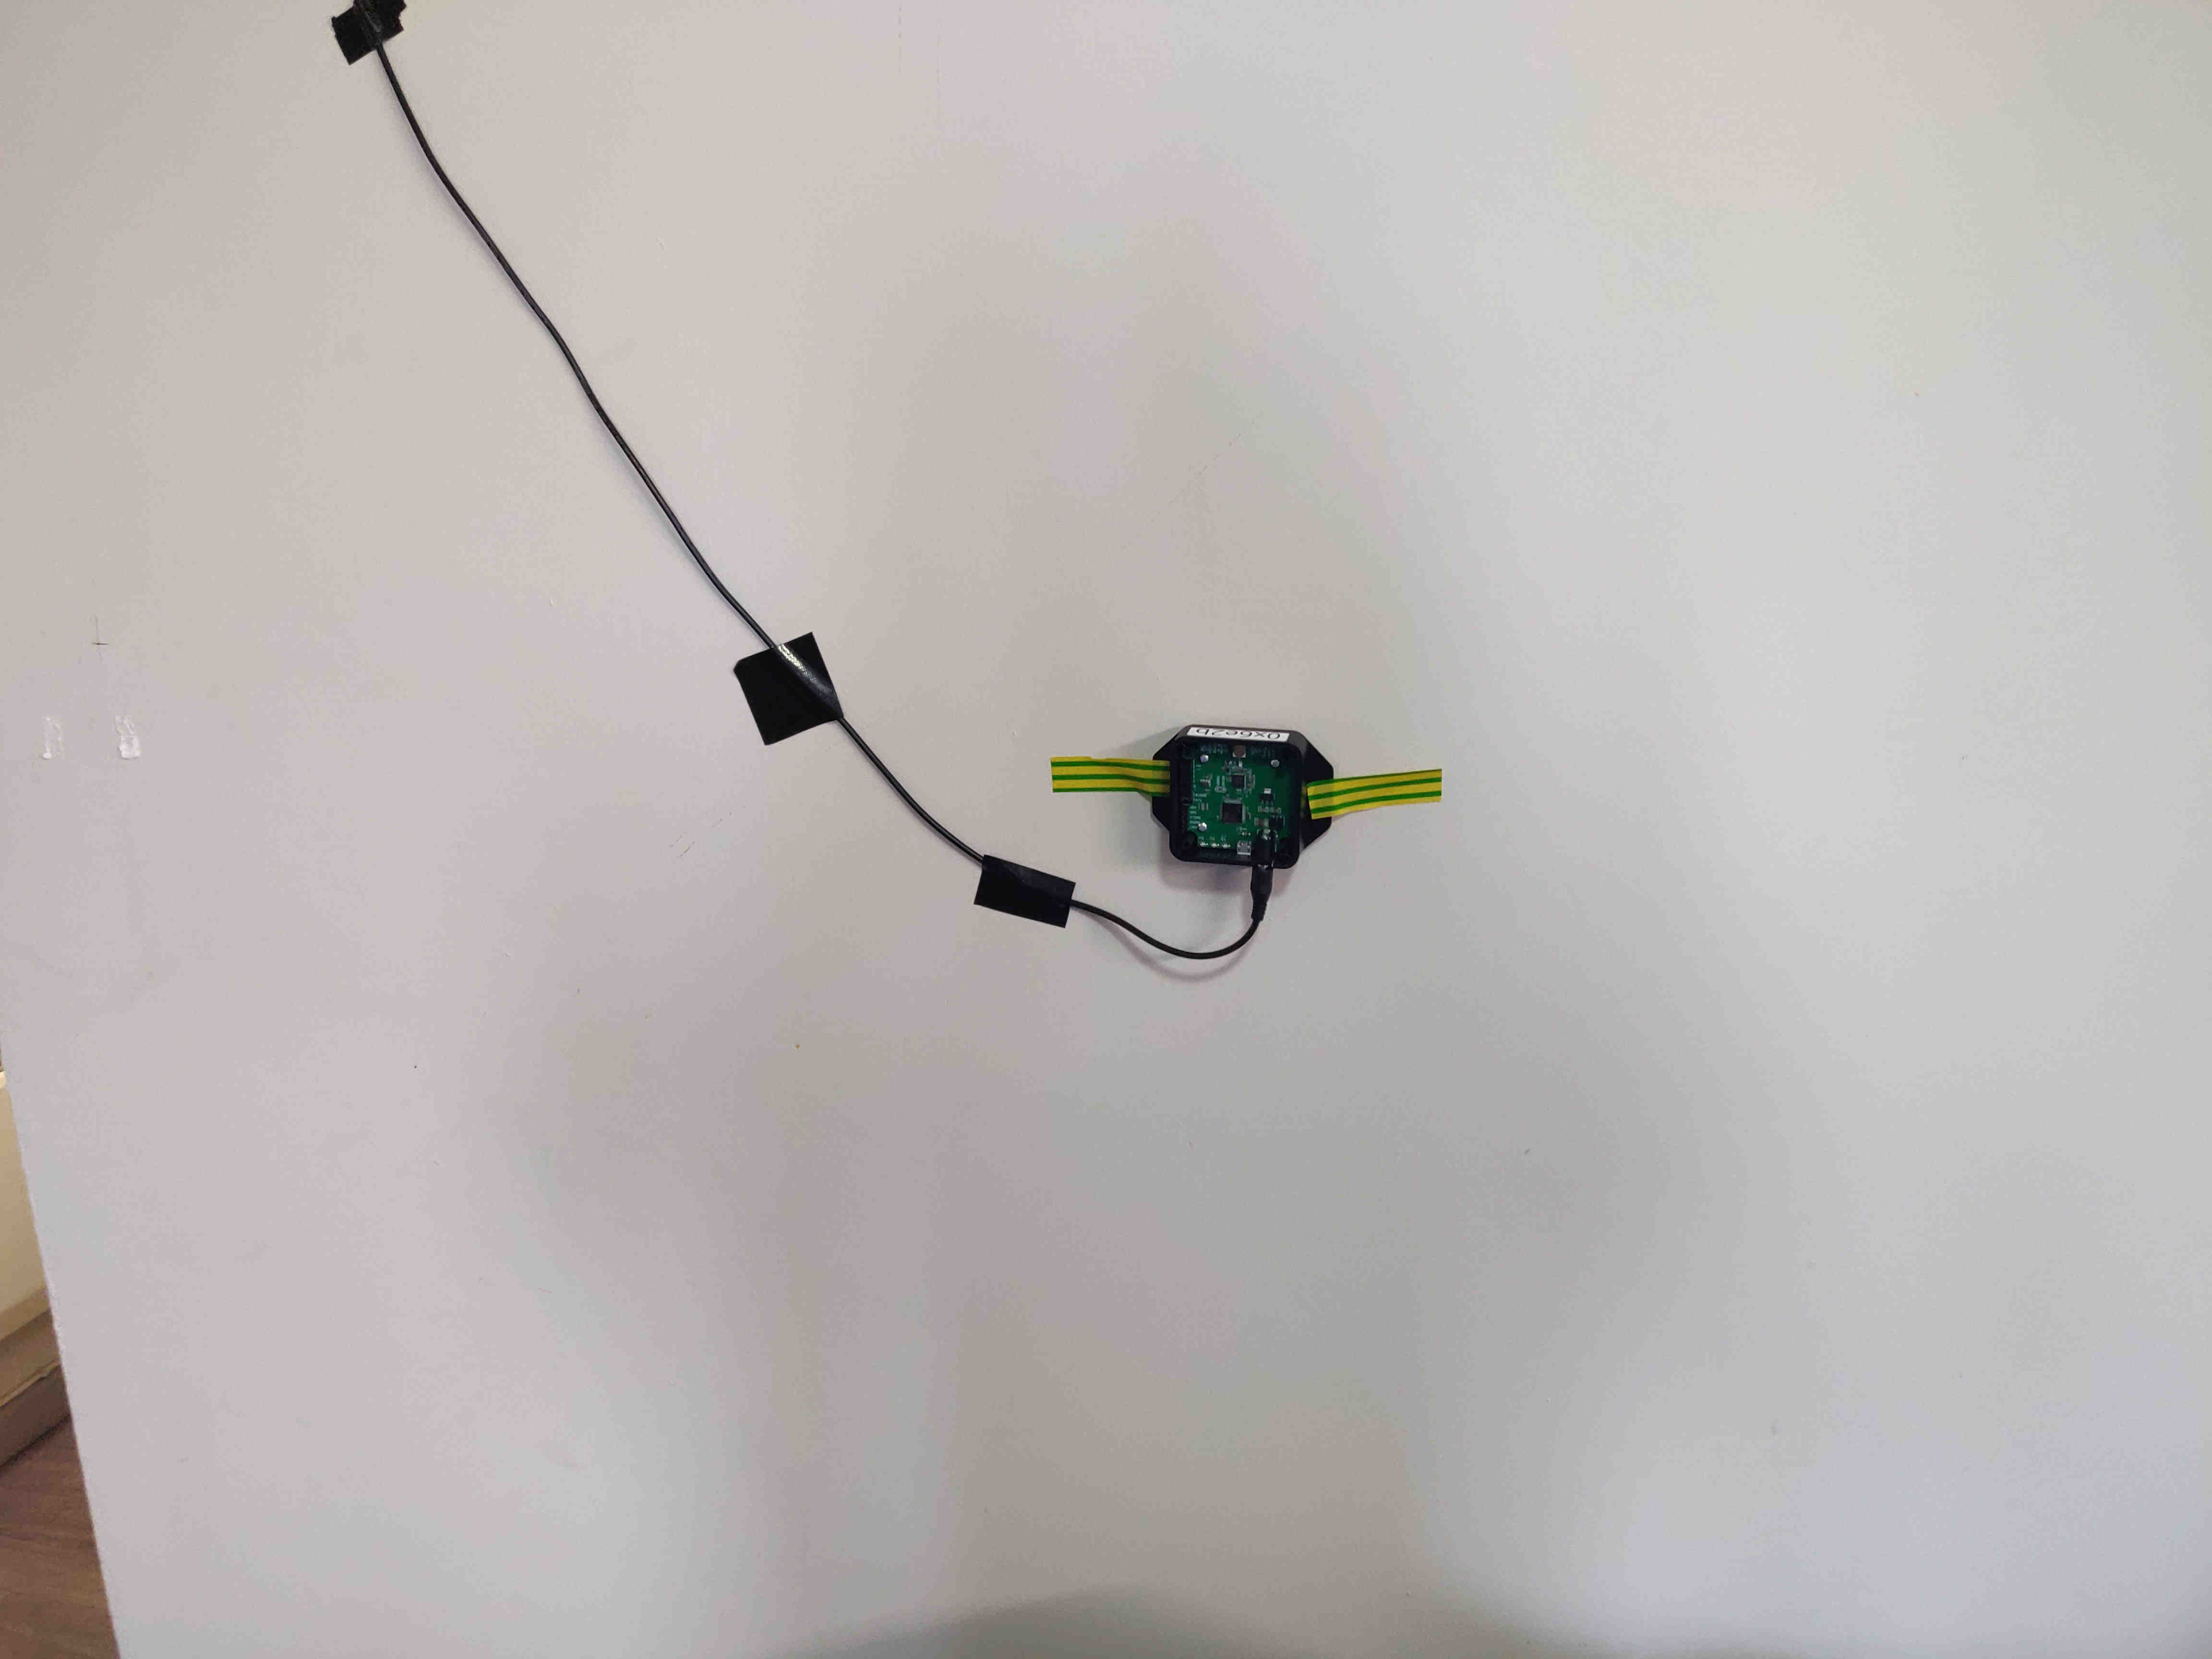
\includegraphics[width=\textwidth]{mtd/anchor1}
            \caption{Anchor 1}
    \end{subfigure}
    \begin{subfigure}[b]{0.4\textwidth}
            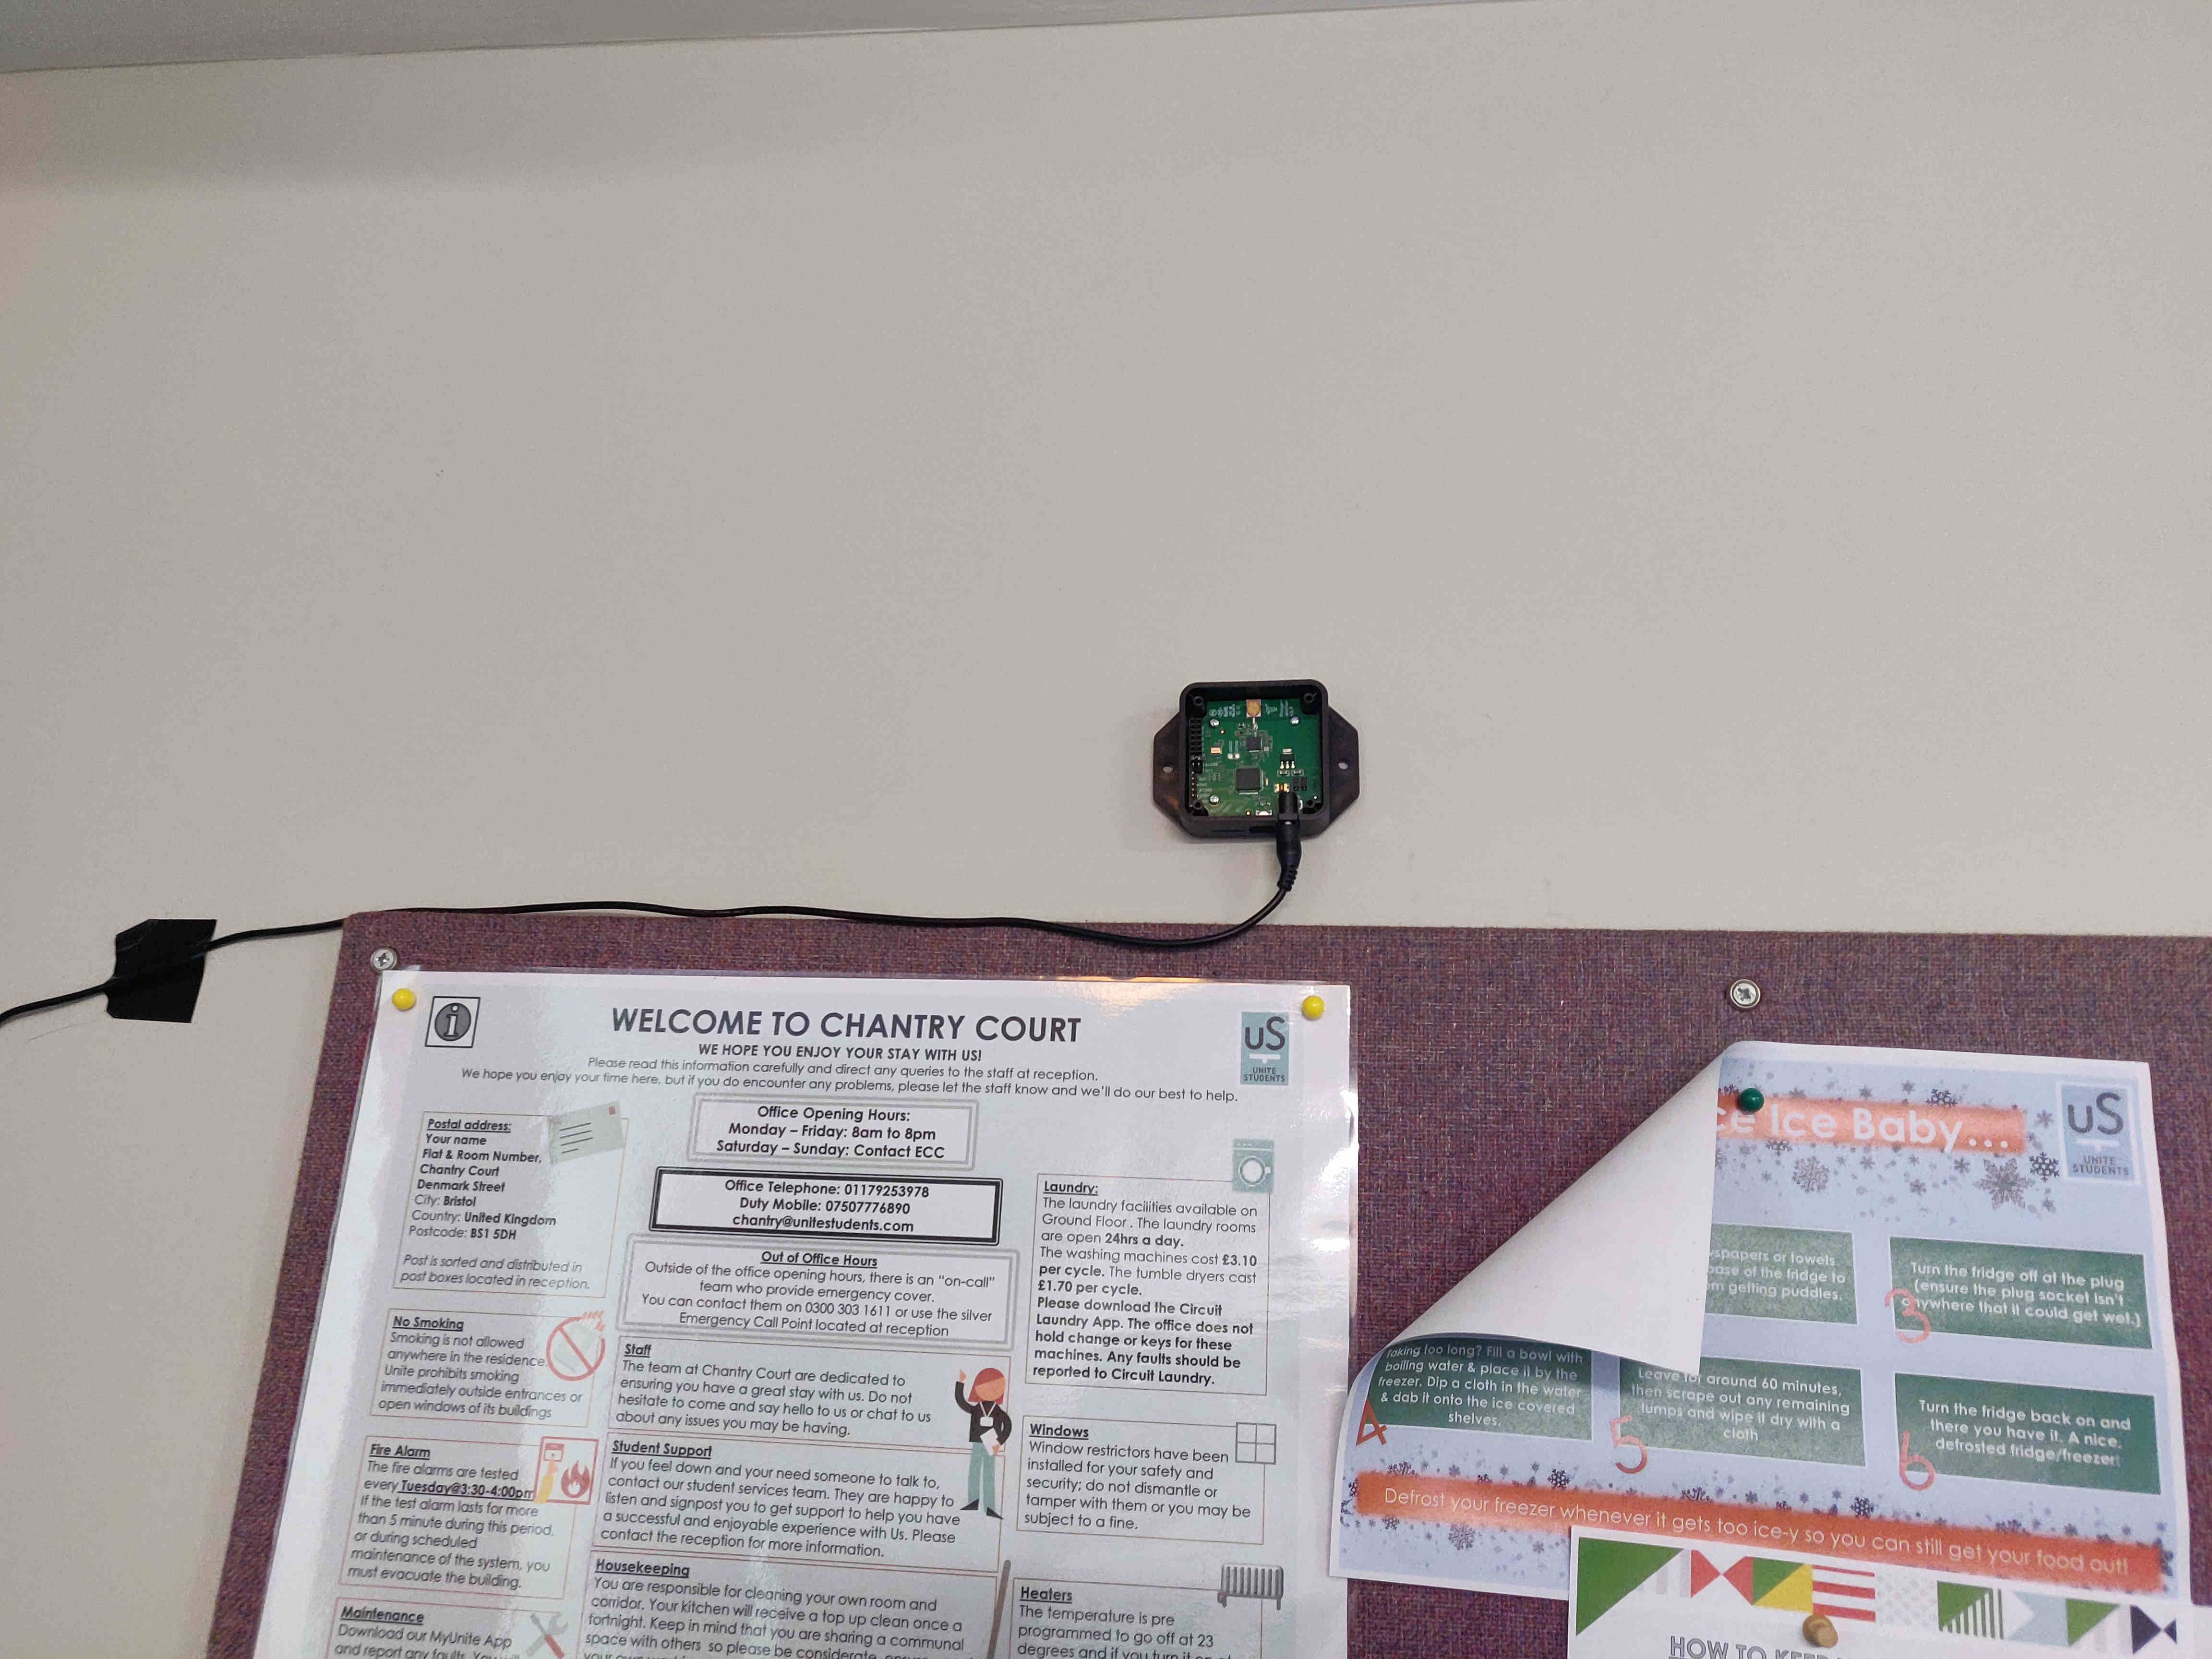
\includegraphics[width=\textwidth]{mtd/anchor2}
            \caption{Anchor 2}
    \end{subfigure}

    \begin{subfigure}[b]{0.4\textwidth}
            \includegraphics[width=\textwidth]{mtd/anchor3}
            \caption{Anchor 3}
    \end{subfigure}
    \begin{subfigure}[b]{0.4\textwidth}
            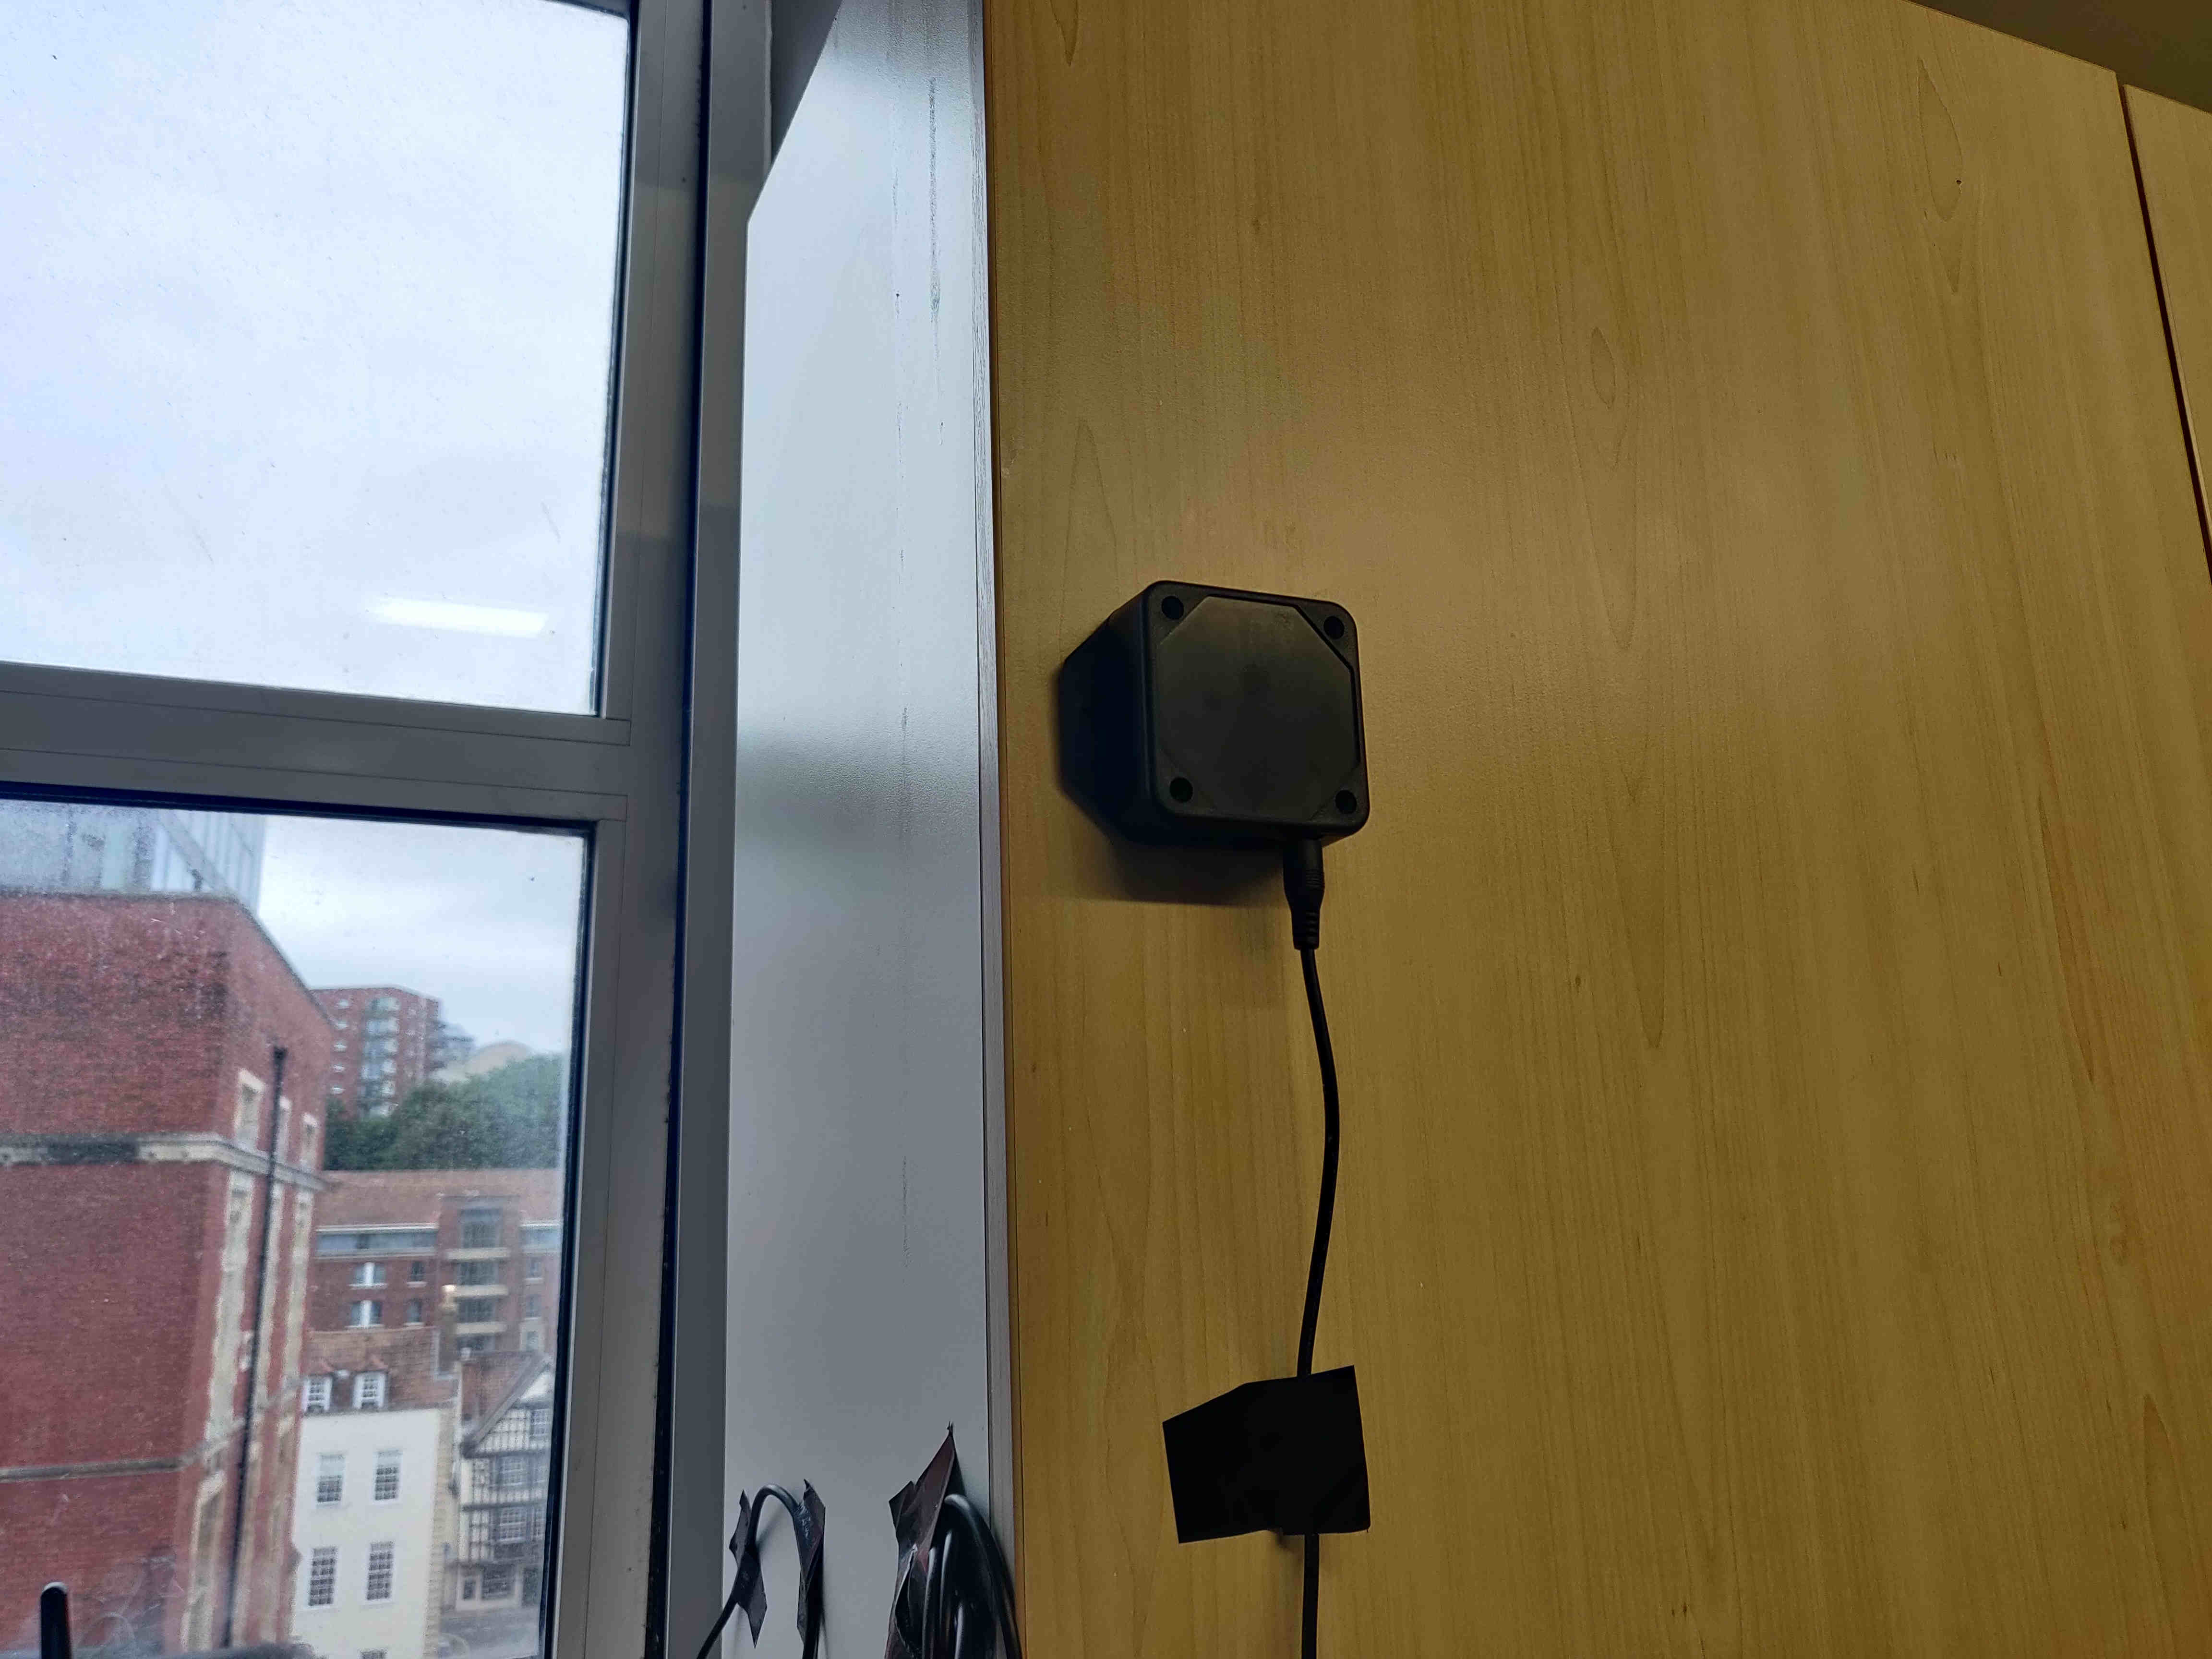
\includegraphics[width=\textwidth]{mtd/anchor4}
            \caption{Anchor 4}
    \end{subfigure}

    \begin{subfigure}[b]{0.7\textwidth}
            \includegraphics[width=\textwidth]{mtd/kitchen_full}
            \caption{Actual Kitchen Layout}
    \end{subfigure}
    \caption{Physical layout of the kitchen/Test Area}
    \label{fig:kitchen}
\end{figure}
\medskip
Figure: ~\ref{fig:kitchen} shows the physcial locations of the pozyx anchors with respect to obstacles in the environment.
Some things to note are:
\begin{itemize}
    \item The walls are made from concrete and dry wall and there are no underlying materials that affected the performance of the anchors.
    \item The fridges have dimensions of $(600*600*1750)$mm.
    \item The corner of the island is located at $(1525,2106,918)$ and it has a dimension of $(2450*900*918)$mm.
    \item Above the island is considered traversible while beneath it will be considered to be impossible to traverse to simply future experiments.
\end{itemize}
%TODO: Insert the pics I took of the anchors here.
%Intro to the basic concept, highlight Pietra's paper and how I am using that to phrase and determine the best location
%Show pics, diagrams and initial table of results?

\subsection*{Summary}
The initial results allowed for a suitable configuration to be obtained but results were recorded in an ideal scenario.
Although these provide a good baseline for what to expect under good operational conditions, the parameters and limitations of the system would need to be tested before any form of optimisation
and improvement to position estimates can be done.
In the next Section: ~\ref{sec:op-params} we investigate this.

\newpage
\section{Operational Parameters}\label{sec:op-params}
%\lipsum[2-4]
As mentioned in the Section:~\ref{sec:anchor-configurations} the best anchor configurations for the given environment was determined  but the results were collected in an ideal scenario.
From work done by ~\citet{evaluwb} it was seen that the major factor affecting the positional accuracy seems to be No Line Of Sight (NLOS) between the anchors and a tag at any given time.
                            %^TODO: Mention this in LR also?
Furthermore, the work discusses the use of using an optimal triplet of anchors in order to improve accuracy.
This is an indication that a loss of a single anchor in the optimal configuration determined in the previous section should still yield reasonable results.
To confirm the operational parameters the following experiments were carried out.

\subsection{Loss of Anchor}\label{subsec:loss-of-anchor}
In theory, a minimum of three anchors are all that is needed for determining the two-dimensional position, $(x,y)$, of the tag via trilateration.
Losing a single anchor would, therefore, allow for the $(x,y)$ position to be determined with a fair amount of accuracy with discrepancies showing up in the z position readings.
To test this, data was recorded, starting with all four anchors and then systematically one anchor was turned of in each sample.
Figure~\ref{fig:Loss_anchors} shows the plots obtained under this test.
It can be seen that the $(x,y)$ position remains relatively unchanged in all with only a notable shift the z position with the loss of Anchor 1 and more noise introduced with the loss of Anchor 4.

\begin{figure}[h!]
    \centering
    \begin{subfigure}{0.45\textwidth}
            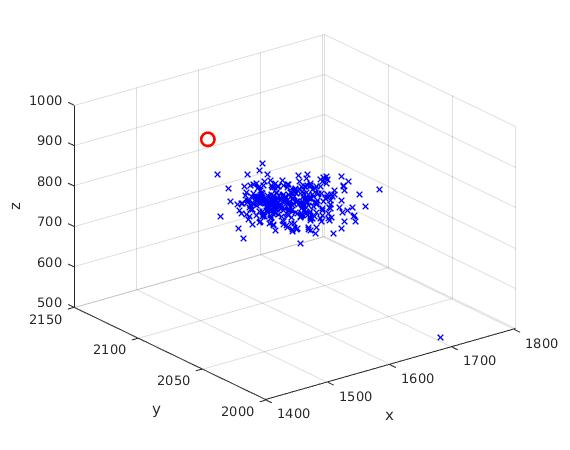
\includegraphics[width=\textwidth]{results/lossanchor1}
            \caption{Loss of Anchor 1}
    \end{subfigure}
    \begin{subfigure}{0.45\textwidth}
            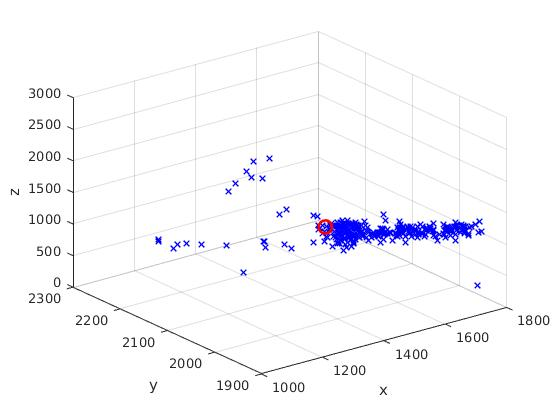
\includegraphics[width=\textwidth]{results/lossanchor2}
            \caption{Loss of Anchor 2}
    \end{subfigure}

    \begin{subfigure}{0.45\textwidth}
            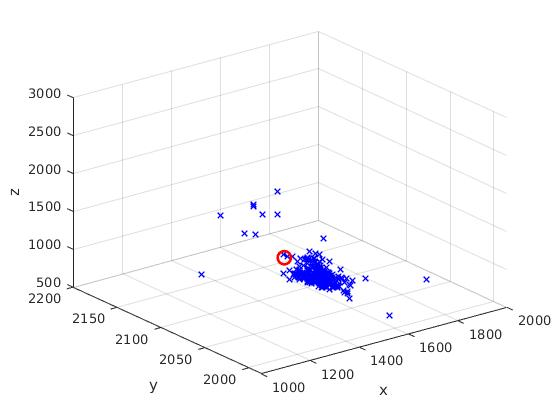
\includegraphics[width=\textwidth]{results/lossanchor3}
            \caption{Loss of Anchor 3}
    \end{subfigure}
    \begin{subfigure}{0.45\textwidth}
            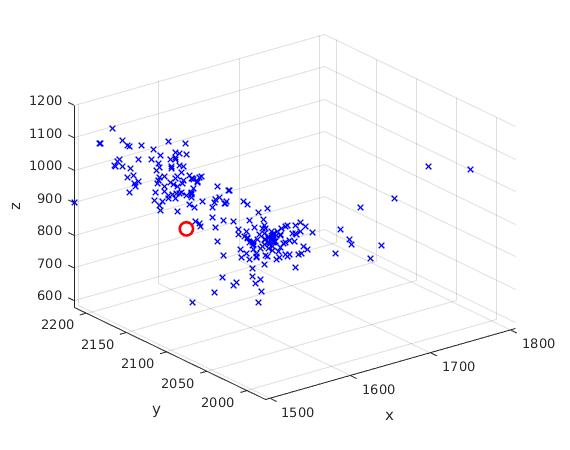
\includegraphics[width=\textwidth]{results/lossanchor4}
            \caption{Loss of Anchor 4}
    \end{subfigure}
    \caption{Results obtained when an Anchor was lost.}
    \label{fig:Loss_anchors}
\end{figure}
\newpage
\subsection{No Line of Sight}\label{subsec:no-line-of-sight}
The positioning calculations are based on a Two way ranging and Time of flight calculation scheme (see Appendix~\ref{app:app01}).
The major crux of the calculation is that the wave is always moving at the speed of light this means that introducing an obstacle between any anchor and the tag that attenuates the signal would introduce discrepancies in the results obtained.
Figure~\ref{fig:nlos} shows the setup used to test this scenario.
The system was allowed to record data with no obstacles then a person walked along the trajectory indicated by the dotted arrows in the Figure and came to a rest as seen.
It was ensured that the path taken by the person did not obstruct any of the anchors during motion.
This was carried out 3 times:
\begin{enumerate}
    \item Position 1: Provides NLOS between Anchor 2 and the tag.
    \item Position 2: Does not provide NLOS between any anchors and the tag.
    \item Position 3: Provides NLOS between Anchor 4 and the tag.
\end{enumerate}
Position 2 was done to confirm that no reflections or attenuation occur with a person just being in the proximity of the tag.
From Figure~\ref{fig:persons} we can see that a person being introduced at position 1 obstructs the line of sight between an anchor and the tag and has adverse effects.
It is clear that the 2 distinct blobs seen in the plots for position 1 and 3 show that the tag's 'position' has changed although it is stationary.

\begin{figure}[h!]
    \centering
    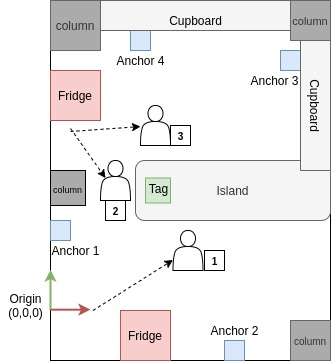
\includegraphics{mtd/loss_of_ppl}
    \caption{The test scenario for No Line of Sight experiment}
    \label{fig:nlos}
\end{figure}

\begin{figure}[h!]
    \centering
    \begin{subfigure}{0.45\textwidth}
            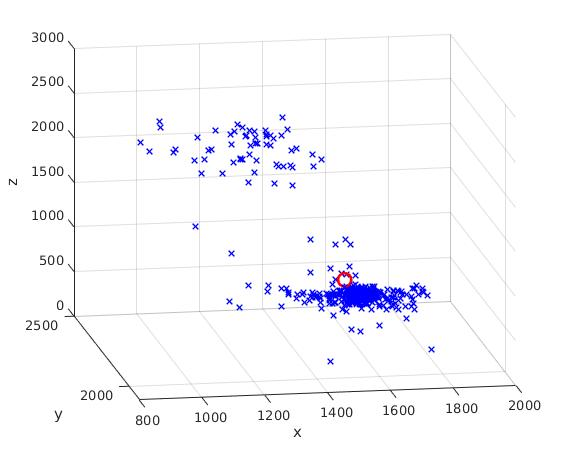
\includegraphics[width=\textwidth]{results/personatposition1}
            \caption{Person at Position 1}
    \end{subfigure}
    \begin{subfigure}{0.45\textwidth}
            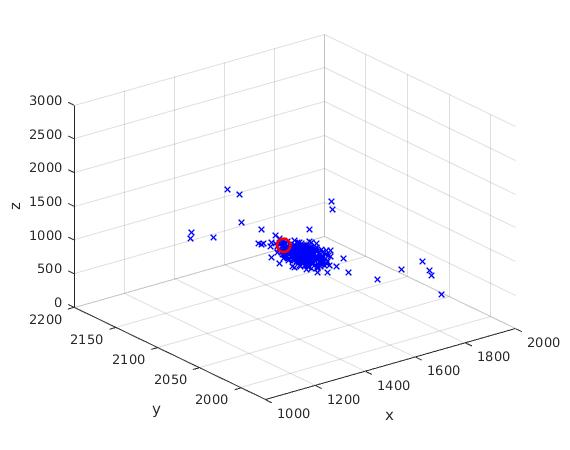
\includegraphics[width=\textwidth]{results/personatposition2}
            \caption{Person at Position 2}
    \end{subfigure}
    \begin{subfigure}{0.45\textwidth}
            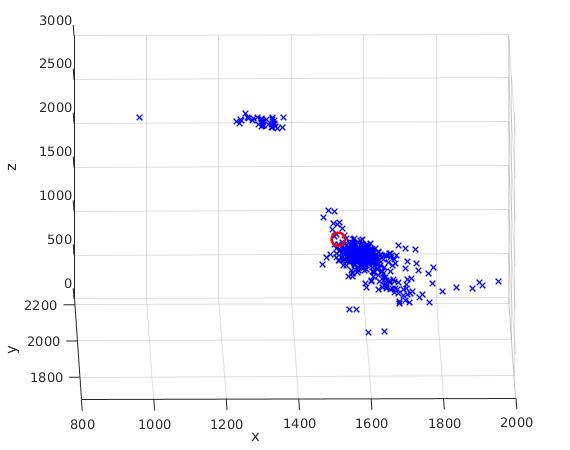
\includegraphics[width=\textwidth]{results/personatposition3}
            \caption{Person at Position 3}
    \end{subfigure}
    \caption{Results obtained when a person provides No Line of Sight.}
    \label{fig:persons}
\end{figure}
As it stands, NLOS is the major factor affecting the operation of the system and the accuracy of the raw readings.
As such it was proposed that additional layers be added to process this positional data in order to improve the accuracy of the system and make it robust.


\newpage
\section{Technical Design}\label{sec:technical-design}
\lipsum[2-8]